%%%%%%%%%%%%%%%%%%%%%%%%%%%%%%%%%%%%%%%%%%%%%%%%%%%%%%%%%%%%%%%%%%%%%%%%%%%%%%%%
% IMU Odometry Challenge — Technical Report (team Lexxxxx), template 2026-09-04
%%%%%%%%%%%%%%%%%%%%%%%%%%%%%%%%%%%%%%%%%%%%%%%%%%%%%%%%%%%%%%%%%%%%%%%%%%%%%%%%
\documentclass[letterpaper,10pt,conference]{ieeeconf}
\IEEEoverridecommandlockouts
\overrideIEEEmargins
\usepackage{amsmath}
\usepackage{amssymb}
\usepackage{booktabs}
\usepackage{multirow}
\usepackage{array}
\usepackage{tabularx}
\usepackage{xcolor}
\usepackage{url}
\usepackage{hyperref}
\hypersetup{colorlinks=true, urlcolor=red, linkcolor=black, citecolor=black}
\def\UrlBreaks{\do\/\do\_\do\.}
\usepackage{graphicx}
\usepackage{tikz}
\usetikzlibrary{arrows.meta,positioning,fit,calc}
\urldef{\scoringurl}\url{https://huggingface.co/spaces/Tartan-IMU/imu_odometry_challenge_scoring}
\newcommand{\vdr}{v_{\mathrm{DR}}}

\title{\LARGE \bf Technical Report for the IMU Odometry Challenge}
\author{\\
One Unified Inertial Velocity Model with Learned Calibration Channels,\\a Gated Physics Recursion and Drag-Consistent Augmentation\\
Kaggle team name: \textcolor{red}{\textit{Lexxxxx}}\\
Hao-Ting Ho$^{1}$%
\thanks{$^{1}$Hao-Ting Ho is with the Department of Electrical Engineering, Tunghai University,
        Taichung, Taiwan (e-mail: {\tt\small haoting.ho@outlook.com}; {\tt\small lexho2005@gmail.com}).}%
}

\begin{document}
\maketitle
\thispagestyle{empty}
\pagestyle{empty}

%%%%%%%%%%%%%%%%%%%%%%%%%%%%%%%%%%%%%%%%%%%%%%%%%%%%%%%%%%%%%%%%%%%%%%%%%%%%%%%%
\begin{abstract}
We submit one network with one set of weights for all four platforms. Its core idea is to give a
compact CNN--GRU velocity regressor the physical quantities a strapdown system would compute, while
never letting them act as a second estimator: two small sub-modules stored in the same checkpoint
calibrate each recording's IMU (accelerometer scale, bias, time constant, gyro-axis map) and
integrate a rest-anchored attitude, from which a bounded dead-reckoned velocity, the time since the
rest anchor and the rotation to the anchor frame enter the network as input channels. A dilated
1-D ResNet encodes each 1-s window into five tokens, a bidirectional GRU over 40 windows supplies
context, and the velocity is read out by a direct head combined with a learned-gain recursion over
the window-to-window IMU increments. The trunk is initialised by masked-IMU self-supervised
pre-training on the released train+val IMU; the training augmentation that matters most is a
drag-consistent translation scaling (``S-fast'') of the racing-quadrotor family, which moves the
fast-sprint tail of the test set. Only the released train and validation splits are used; inference
is deterministic, offline within one trajectory, without platform labels, ensembling, test-time
augmentation or adaptation. On the official full-test scoring service the submission scores
\textbf{0.25878} (ATE$_{20}$ 0.617\,m, AVE 0.220\,m/s; public leaderboard 0.32793). A second,
simpler entry without the inertial channels but with a recording-level FiLM scores 0.26306. We
report the seed range, the three-population structure of our validation protocol, and a quantified
negative result on the recursion gain.
\end{abstract}

%%%%%%%%%%%%%%%%%%%%%%%%%%%%%%%%%%%%%%%%%%%%%%%%%%%%%%%%%%%%%%%%%%%%%%%%%%%%%%%%
\section{Introduction}

\textbf{Challenges.} A 1-s window of 6-axis IMU determines body velocity only weakly. On this
benchmark~\cite{imuchallenge} three facts dominate. (i) Sensor error is decisive within one second: integrating the raw
accelerometer with ground-truth gravity and ground-truth initial velocity gives a validation AVE of
0.66\,m/s after 1\,s (learned model 0.22) and grows linearly (2.2 at 5\,s, 7.0 at 20\,s), so any
``physics plus learned correction'' scheme has the roles reversed --- the network is the estimator
and physics can only supply features. (ii) The drone data are two sources: 43 of 282 training
recordings have an IMU frame equal to the label frame, the other 239 are ``upside down plus a
recording-specific yaw offset'', with a 10$\times$ different noise floor; the error of every model
we trained concentrates on the identity-frame source (fast, noisy, short flights). (iii) The test
split is deliberately faster than train: four straight-sprint sequences (\#29, \#56, \#37, \#38)
carry 43\,\% of the drone AVE, and drone carries 68\,\% of the score.

\textbf{Motivation.} The released 4-head TartanIMU baseline~\cite{tartanimu} needs the platform label at inference and scores
0.937 on the anonymised test set under any label-free head selection, so a genuinely unified model
had to be trained from scratch. Validation, in turn, is blind to the sprint tail (no validation
trajectory exceeds 10\,m/s), so the second half of our work was as much about building rulers that
see the tail as about models.

\textbf{Key components.} Dense random-offset windowing; a dilated 1-D ResNet with five tokens per
window; a bidirectional GRU over 40 consecutive windows with a 5-s low-pass side branch; an
8-channel decomposition about a slow complementary-filter ``up''; masked-IMU self-supervised
pre-training of the trunk; physics-consistent time dilation and drag-consistent translation scaling
as augmentation; per-recording calibration (CalNet) and attitude (AttNet) sub-modules producing
inertial input channels; and a learned-gain recursion head.

\textbf{What we think is worth reporting.} (a) S-fast: scaling the gravity-removed specific force
and the velocity labels jointly on the racing family, the first of $\approx$30 interventions we
measured that moved the sprint tail (summed tail AVE 15.1$\to$12.7\,m/s; the inertial channels then
take it to 11.8). (b) Physics inside the network rather than after it: the inertial quantities are
channels and increments, the only velocity output is the network's. (c) An evaluation protocol that
treats validation, a high-rotation fold and a sprint fold as three different populations and uses
each as a gate rather than a ranker. None of these is new in isolation; what we can offer is a
measured account of how far each one goes on this benchmark.

\textbf{Contributions.} Beyond the model, the report is organised as a record of eight
investigations (Sec.~\ref{sec:devexp}), each stating what we measured, what we decided on it, and
where the outcome differed from what we expected: the location of the error, memorisation and
self-supervised pre-training, physics-consistent time dilation, the construction of rulers that
see the sprint tail, the drag mechanism behind S-fast, the learned inertial channels, the
recursion gain, and data scale. Three of these ended in quantified negative results, which we
report at the same level of detail as the positive ones; the ablation chain on the official full
test (0.2702 $\to$ 0.2658 $\to$ 0.2588) is given with seed ranges.

%%%%%%%%%%%%%%%%%%%%%%%%%%%%%%%%%%%%%%%%%%%%%%%%%%%%%%%%%%%%%%%%%%%%%%%%%%%%%%%%
\section{Method}

\subsection{Overall Architecture}
Fig.~\ref{fig:method_overview} shows the pipeline; every box runs once per recording or per chunk
and is part of one checkpoint. \emph{Per recording}: CalNet maps a 64-d summary of the raw IMU
(rest statistics, gravity-norm consistency, low-passed tilt consistency) to an accelerometer scale
$S\in\mathbb{R}^3$, bias $b$, time constant $\tau$ and a gyro-axis map class; the calibrated IMU
feeds AttNet, a rest-anchored SO(3) gyro integration (parallel prefix products of small-angle
blocks) with GRU-predicted corrections, giving $R_{t\to F_0}$. From these we derive the rest-frame
up direction, a bounded dead-reckoned velocity $\vdr = q\tanh(\int (R f_{\rm cal}+g)\,dt/q)$ with
$q=8$\,m/s, the time since the rest anchor and the first two columns of $R_{t\to F_0}$.
\emph{Per window}: 25 input channels (raw IMU 6, complementary-filter decomposition 8, rest
reference 4, rest-up 3, $\vdr$ 3, time since anchor 1) enter a dilated 1-D ResNet (7 residual
blocks, 192 channels, 25 steps) that is pooled into five tokens with a phase embedding.
\emph{Per chunk}: a two-layer bidirectional GRU over $K=40$ windows plus a ``wide'' branch (5-s
low-pass summary of the block) produces per-window features $h_k$. \emph{Heads}: a linear direct
head $v^{\rm d}_k$, and a recursion
\begin{equation}
v_k = \Delta R_k v_{k-1} + \Delta V_k + K_k\,(v^{\rm d}_k - \Delta R_k v_{k-1} - \Delta V_k),
\label{eq:ekf}
\end{equation}
where $\Delta R_k,\Delta V_k$ are the gyro/calibrated-accelerometer increments between window
ends and $K_k=\sigma(W[h_k;\,t_{\rm since};\,s_{\rm rest};\,\log(1+\|\vdr\|)])$ is a learned
3-vector gain (bias $+3$, i.e.\ it starts as the direct head). An auxiliary platform-logit head is a
training regulariser only and is discarded at inference. Nothing in the network receives a platform
label or routes to platform-specific parameters; the only platform-dependent behaviour is what the
shared weights infer from the signal. Design choices aimed at cross-platform and
out-of-distribution generalisation: platform-uniform sampling, no per-platform normalisation, the
fixed normalisation of the inertial channels (so that a car's drift cannot inflate the statistics),
the bounded $\vdr$, and augmentation only on the family whose test distribution is under-covered.

\begin{figure}[htbp]
\centering
\resizebox{\linewidth}{!}{%
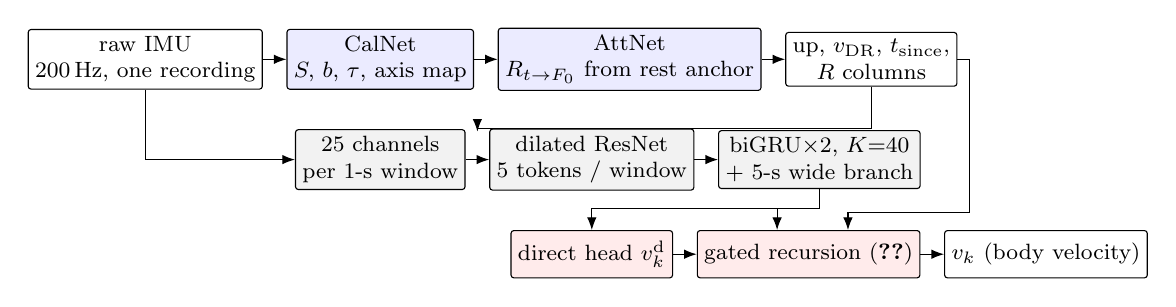
\begin{tikzpicture}[font=\footnotesize, node distance=2mm and 3mm,
  box/.style={draw, rounded corners=1pt, align=center, inner sep=2.5pt, minimum height=6mm},
  sub/.style={box, fill=blue!8}, main/.style={box, fill=gray!10}, hd/.style={box, fill=red!8},
  arr/.style={-{Latex[length=1.6mm]}, thin}]
\node[box] (imu) {raw IMU\\200\,Hz, one recording};
\node[sub, right=of imu] (cal) {CalNet\\$S,\,b,\,\tau$, axis map};
\node[sub, right=of cal] (att) {AttNet\\$R_{t\to F_0}$ from rest anchor};
\node[box, right=of att] (der) {up, $\vdr$, $t_{\rm since}$,\\$R$ columns};
\node[main, below=5mm of cal] (ch) {25 channels\\per 1-s window};
\node[main, right=of ch] (res) {dilated ResNet\\5 tokens / window};
\node[main, right=of res] (gru) {biGRU$\times$2, $K{=}40$\\+ 5-s wide branch};
\node[hd, below=5mm of res] (dh) {direct head $v^{\rm d}_k$};
\node[hd, right=of dh] (ekf) {gated recursion (\ref{eq:ekf})};
\node[box, right=of ekf] (v) {$v_k$ (body velocity)};
\draw[arr] (imu)--(cal); \draw[arr] (cal)--(att); \draw[arr] (att)--(der);
\draw[arr] (imu.south) |- (ch.west);
\draw[arr] (der.south) |- ($(ch.north east)!0.5!(res.north west)$) -- ($(ch.north east)!0.5!(res.north west)+(0,-1pt)$);
\draw[arr] (ch)--(res); \draw[arr] (res)--(gru);
\draw[arr] (gru.south) -- ++(0,-2.5mm) -| (dh.north);
\draw[arr] (gru.south) -- ++(0,-2.5mm) -| ($(ekf.north)+(-4mm,0)$);
\draw[arr] (dh)--(ekf); \draw[arr] (ekf)--(v);
\draw[arr] (der.east) -- ++(1.5mm,0) |- ($(ekf.north)+(5mm,2.2mm)$) -- ($(ekf.north)+(5mm,0)$);
\end{tikzpicture}}
\caption{The submitted pipeline. Blue: per-recording sub-modules trained on released labels and
frozen inside the same checkpoint. Grey: the velocity network. Red: the two heads; the recursion
uses the increments $\Delta R_k,\Delta V_k$ between window ends, and the fused $v_k$ is the only output.}
\label{fig:method_overview}
\end{figure}

\subsection{Data Processing}
\textbf{Preprocessing.} Raw 6-axis IMU at 200\,Hz in the body frame with gravity retained; no
resampling. A complementary filter ($\alpha=0.005$) estimates the body-frame up direction and gives
eight channels (specific force and angular rate split along/about up). CalNet applies
$f_{\rm cal}=S\odot(f-b)$ with a $\tau$ time shift of the gyro and, for the second drone source, a
fixed axis map; AttNet supplies $R_{t\to F_0}$ from the calmest 1-s window (minimum
$|\overline{\|a\|}-g|+\overline{\|\omega\|}+0.5\,\mathrm{std}\|a\|$). Channels are standardised
with train statistics except the inertial ones (fixed scale 5\,m/s and 10\,s). Training windows are
drawn at random 200-frame offsets (dense sampling) in chunks of 40 consecutive windows that never
cross a trajectory boundary; inference uses the fixed non-overlapping windows of the index with
chunks at stride 20 and takes, for each window, the chunk whose centre is nearest.

\textbf{Augmentation (physically motivated).} (1) Time dilation on drone segments ($p=0.5$):
resample by $k\sim U(0.7,1.5)$, $\omega'=k\omega$, $v'=kv$, $f'=k^2(f-g\,\hat u)+g\,\hat u$ with
$\hat u$ the ground-truth up (training only); for the identity-frame racing family $k\le1.2$.
(2) \emph{S-fast}: for the racing family only, drawn instead of (1) on half of the augmented
samples, a translation scaling $s\sim U(1.0,1.8)$: $f'=s(f-g\,\hat u)+g\,\hat u$, $v'=sv$, gyro and
attitude unchanged --- the specific-force/velocity relation of straight flight at higher speed with
the same drag law. (3) Direction-only yaw augmentation about the estimated up ($p=0.5$) for the
identity source. (4) Random dropout of the inertial channels ($p=0.3$) so the network never depends
on them alone. Inertial channels are rescaled consistently ($\vdr\cdot ks$, $t_{\rm since}/k$).

\subsection{Training Data}
Table~\ref{tab:datasets} lists everything that touched the submitted model. No external dataset,
synthetic data, pretrained checkpoint or pseudo-label enters it. During development we ran, and
disclose, three excluded lines: (a) one early branch pre-trained on train+val+test raw IMU (scored
once on 9/13, excluded the next day, no derived weights); (b) supervised fine-tuning with the public
NeuroBEM quadrotor dataset after removing segments cross-correlating with competition recordings
(scored on both services, excluded following the organisers' ruling in discussion \#737628);
(c) the public UZH-FPV set, found to coincide with competition recordings including test ones and
deleted unused. Train/val were kept as released for selection; the final models are fit on both.

\begin{table}[htbp]
\centering\footnotesize
\caption{Datasets used for model development and training.}
\begin{tabular}{p{2.1cm} p{1.0cm} p{4.3cm}}
\toprule
Dataset & Type & Usage \\
\midrule
Challenge train (395 traj.) & Official & Supervised training; SSL pre-training (IMU only); CalNet/AttNet targets \\
Challenge val (80 traj.) & Official & Selection during development; folded into the final fit \\
Challenge test (89 traj.) & Official & Raw-input inference only \\
NeuroBEM, UZH-FPV & Public & Development experiments only; \textbf{not} in the submitted model \\
\bottomrule
\end{tabular}
\label{tab:datasets}
\end{table}

\subsection{Training and Optimization}
Loss: vector Huber ($\beta=0.05$) on the fused output, $0.5\times$ the same on the direct head,
$0.5\times$ binary cross-entropy teaching the gain which of $v^{\rm d}_k$ / propagation is closer to
the label, and $0.05\times$ platform cross-entropy. AdamW, lr $2\times10^{-3}$, OneCycle,
120 epochs $\times$ 160 steps, batch 52 chunks $\times$ 40 windows, dropout 0.2, AMP.
Stages: (i) masked-IMU pre-training of the trunk on train+val IMU (dense windows, 60 masked frames
$\times$ 14 channels, 3\,h); (ii) CalNet (1\,min) and AttNet (4\,min) on train+val labels, then
frozen; (iii) the velocity network, 120 epochs on train+val ($\approx$30\,min on an RTX 5090).
No curriculum, domain adaptation or platform specialisation. The submitted checkpoint is the fixed
last epoch; the seed (42) was designated before any seed of this recipe was scored. Development used
train-only twins of every recipe with val as the selection metric plus two stress folds of the
training split (Sec.~\ref{sec:devexp}).

\subsection{Inference}
\texttt{predict.py} reads \texttt{index/test\_windows.csv} and \texttt{test/*.npz}, and for every
recording runs CalNet $\to$ AttNet $\to$ derived channels $\to$ chunked network $\to$ recursion, then
writes one body-frame velocity per window. It is offline and non-causal within one trajectory
(40-s bidirectional context, recording-level sub-modules), deterministic, single pass, no
test-time augmentation, ensembling, smoothing, rescaling or adaptation; the development-time and
submitted pipelines are the same code. Throughput on CPU: 30,644 windows in 85\,s (360 windows/s);
on one GPU under one minute.

\subsection{Model Complexity and Runtime}
Table~\ref{tab:runtime}. The method cannot run online as submitted (it needs future context and the
whole recording for the sub-modules); a causal variant would need a causal GRU and a running
anchor.

\begin{table}[htbp]
\centering\footnotesize
\caption{Model complexity and runtime statistics.}
\begin{tabular}{lc}
\toprule
Property & Value \\
\midrule
Parameters & 2,166,242 (+77,585 sub-modules) \\
Training hardware & 1$\times$ RTX 5090 (final fit) \\
Training time & 3\,h SSL + 5\,min sub-modules + 30\,min \\
Inference hardware & CPU (verified) or one GPU \\
Inference speed & 360 windows/s (CPU); test set 85\,s \\
Peak memory & 2.0\,GB RSS (CPU); $<$1\,GB VRAM (GPU) \\
\bottomrule
\end{tabular}
\label{tab:runtime}
\end{table}

%%%%%%%%%%%%%%%%%%%%%%%%%%%%%%%%%%%%%%%%%%%%%%%%%%%%%%%%%%%%%%%%%%%%%%%%%%%%%%%%
\section{Development Experiments}
\label{sec:devexp}
We organise the record as eight investigations. Each states what we measured, what came out, what
we decided, and where the outcome differed from what we expected. Numbers are val (released
split, official scorer) unless marked \emph{official} (89-sequence full test). Differences below
$\pm$0.006--0.011 (seed-paired bootstrap, 2--8 seeds) were not interpreted.

\textbf{1. Where the error is.} \emph{Measured:} the first official per-sequence decomposition
(all3, 9/12); the test recordings assigned to platforms by the auxiliary head (its 45/2099 drone
count matched the organisers' table exactly); IMU statistics of train, val and test per platform.
\emph{Result:} car, dog and human were \emph{easier} on test than on val (AVE 0.066/0.078/0.058
vs 0.091/0.086/0.069); the entire val$\to$test gap was drone (0.844 vs 0.412), which is 72\,\% of
the score; test drone specific force deviates from gravity 2.9$\times$ more than val. Two days
later the drone data split by noise floor into two sources (10$\times$ apart) with different
IMU/label frame conventions, and the error of every model sat on the identity-frame source
(AVE 0.73 vs 0.33). \emph{Decision:} stop tuning the platforms that were already at val level,
treat drone speed coverage as the only lever, keep one shared model. \emph{Differed from
expectation:} we had assumed the shared model paid for its generality on the slow platforms; the
official table showed the opposite, and the public leaderboard ordered two of our models
oppositely to the full test (a3sslc: public $+$0.0065, full test $-$0.0095), which ended our use of
public score as a signal.

\textbf{2. Memorisation, and the one regulariser that worked.} \emph{Measured:} training Huber
against val for every capacity and context variant; single-platform experts against the shared
model; oversampling of aggressive flights. \emph{Result:} every enlargement (60-window context,
continuous 20-s trunk, longer schedules, 3$\times$ oversampling, a drone expert) cut the training
loss and left val flat or worse; the drone expert equalled the shared model (0.463 vs 0.465)
while fitting three times better. Dropout, weight decay, noise and SAM did not change this.
Masked-IMU reconstruction pre-training of the trunk did ($-0.014$, 3 seeds sd 0.001; 280$\times$
more target values per window than the velocity label), and its gain was largest on the calm
drone subset (0.376$\to$0.332). \emph{Decision:} adopt the pre-trained trunk; stop the capacity
line. \emph{Differed:} scaling the pre-training 3.3$\times$ and a JEPA objective were worse
officially (+0.004, +0.014); the effect saturated at the representation level rather than growing
with compute.

\textbf{3. Physics-consistent time dilation.} \emph{Measured:} replaying drone segments at speed
$k$ with $f'=k^2(f-g\hat u)+g\hat u$, scored by speed quintile and by drone source.
\emph{Result:} $-0.015$ on val with a monotone widening 1.0--1.3 $\to$ 0.7--1.5 and saturation
beyond; the fastest quintile improved 27\,\%; the identity source moved only after a sampler bug
(short recordings never received $k>1$) was fixed ($-7\,\%$). Officially v1 0.2837 $\to$ v2 0.2687.
\emph{Decision:} freeze the range, add nothing on top (S-scaling, 240 epochs, $p=0.75$,
pre-training on dilated data were all within $\pm0.003$). \emph{Differed:} the symmetric range
beat the ``only faster'' range, i.e.\ the gain was not extrapolation but a shape prior; and the
official per-sequence history over 26 models later showed that dilation \emph{raised} the two
17-s sprints by 0.5--1.0\,m/s while lowering the other 41 --- drag grows as $k^2$ and speed as $k$,
so dilated samples teach the wrong tilt-to-speed slope for straight flight.

\textbf{4. Building a ruler that sees the tail.} \emph{Measured:} a 12-recording hold-out
(rerun spread 0.14), then a 26-recording fold with both IMUs of a flight held out together and no
training window above 8\,m/s (spread 0.02--0.04, machine-to-machine offset 0.06, so every machine
carries its own baseline), then a sprint fold that holds out one outdoor sprint pair and keeps the
other sprints in training. \emph{Result:} on the 26-recording fold 15 of 17 interventions
(sampling weights, loss shapes, stronger dilation, increment heads) left the $>8$\,m/s compression
untouched (prediction/truth 0.63--0.68); yaw supervision plus speed-density reweighting passed the
fold ($-0.072$), was trained on train+val, and scored \emph{worse} officially (0.2881 vs 0.2702):
its fold gain came from two side-flying recordings. \emph{Decision:} never rank on a fold; use
each ruler as a gate at twice its seed spread; report per-recording changes, not means.
\emph{Differed:} the fold that held out \emph{all} sprints made rest-reference channels learn the
wrong sign (a large tilt at rest looked ``slow''); the same channels were null on the sprint fold.
The fold design decides what a channel can learn.

\textbf{5. The sprint tail, and S-fast.} \emph{Measured:} a counterfactual probe scaling the
horizontal specific force of \#29/\#56 by 0.5 and 1.5 on our own test predictions (no labels);
IMU statistics of the tail versus the training racing family; the tilt-to-speed slope per training
session. \emph{Result:} v6 and every variant moved by $<0.3$\,m/s under the probe --- the models
did not read drag; the tail is low-thrust, low-rotation straight flight (mean $f_z$ 10.3--10.5,
gyro 0.5\,rad/s) whereas the training racing flights are high-thrust manoeuvres ($f_z$ 11--13,
gyro 0.8--1.9); the session slopes are $-2.5/-3.2/-4.0$. \emph{Decision:} scale specific force
and velocity jointly on the racing family only (S-fast), cap its dilation at 1.2. Sprint fold
2.73 $\to$ 2.10; official 0.2702 $\to$ 0.2658; tail 15.1 $\to$ 12.7. \emph{Differed:} the plan's
own gate (probe sensitivity $\ge1.2$) still failed after S-fast (0.96--1.10), and the first fold
we used rejected it; the decision to continue rested on the redesigned sprint fold and on the
public score, not on the pre-registered gate. A development-time physics readout on the four tail
sequences (nearest session's slope) scored 0.3277 public against v6's 0.3566; it is not part of any
submission, but it told us how much of the gap was this one coefficient.

\textbf{6. Learned inertial channels.} \emph{Measured:} each sub-module against its own oracle
before joint training --- CalNet by a GT-attitude integration of the calibrated accelerometer
(poorly calibrated family 2.4--5.2\,m/s $\to$ 0.17--0.72), AttNet by the up-direction error on
held-out fast flights (0039: 4.4$^\circ\to$1.0$^\circ$); the fusion gate's mean opening per epoch.
\emph{Result:} both sub-modules met their gates, and the first fused model (a3v19) still lost to
S-fast alone on the sprint fold; its gate closed to 0.000 by epoch 30 because only 5\,\% of drone
windows had a trustworthy dead-reckoned velocity; officially it improved drone but leaked into
car (ATE 0.421). A code review found the cause: the unbounded $\vdr$ (car drift of $10^3$\,m/s)
made the channel's normalisation scale $\approx$3000, so the trunk never saw it. \emph{Decision:}
bound $\vdr$ with $q\tanh(\cdot/q)$, fix its normalisation, replace the gate by the recursion
(\ref{eq:ekf}) with 6-D rotation columns and yaw-consistent increments; the result is a3v20,
0.2588. \emph{Differed:} the change was designed for the tail and delivered most of its gain on
human ($-0.057$ ATE) and quadruped; car returned to the band edge rather than to v6.

\textbf{7. What the recursion gain actually does.} \emph{Measured:} 22 train-only cards in one
night with the gain's ``propagation better than direct head'' rate split into windows inside and
outside the 10-s anchor horizon; the mean gain per platform on val; ablations with the increments
removed, rotation only, and the gain trained end-to-end, with a soft target, with a margin, or
forced to the direct head outside the horizon; a three-fold sprint ruler. \emph{Result:} the
integrated-increment variant wins every sprint fold (1.89/1.62/2.40 vs 2.10/1.76/2.49 for S-fast;
removing the increments 2.24, rotation only 2.25) and loses on every platform's val ATE and AVE
(0.1913 vs 0.1784); propagation beats the direct head in 0.8\,\% of windows overall but that
average is diluted by car and human; the val loss scales with the mean gain (gain 1.00: 0.1798,
0.97: 0.1821, 0.60--0.88: 0.189--0.191). \emph{Decision:} keep a3v20 (gain $\approx$0.97) as the
delivery, report the family as a negative result. \emph{Differed:} we expected the in-distribution
loss to come from ``carrying'' outside the horizon; forcing the direct head there did not remove it
(0.1878) --- the loss arises inside the horizon on cars starting from rest, exactly where the
increments are switched on.

\textbf{8. Training data and scale.} Folding val into training: $-0.02$ official. External
quadrotor data (NeuroBEM, cross-correlated segments removed): $-0.006$ on a train-only twin,
$+0.012$ on the train+val model (it substituted for the val fast flights) with a
velocity-proportional $z$-bias on human; excluded by rule. 96 synthetic aggressive flights from
GT differential flatness: $+0.018$ official. Width 1.5$\times$, 60-window context, 240 epochs: flat
or worse. The model is not capacity-limited; it is coverage-limited.

\section{Experiments}

\subsection{Official Challenge Performance}
Tables~\ref{tab:overall_results}--\ref{tab:sequence_results} come from the official scoring
service. Entry A (\texttt{a3v20\_s42}, Kaggle submission 56393290,
\texttt{md5 = \textbf{545d7cddc859a16db045f872251be03c}}) is the primary submission and the released
model; entry B (\texttt{a3v21\_s42}, submission 56393834,
\texttt{md5 = a53e196f6b67e8ea52733f4386b5c403}) is the same network without the inertial
sub-modules and recursion but with a 35-d recording-level FiLM. Public leaderboard: 0.32793 (A),
0.32695 (B); the private leaderboard had not been published when this report was written.

\begin{table}[htbp]
\centering\footnotesize
\caption{Overall challenge performance (official scoring service, all 89 test sequences).
Score $=0.6\,\mathrm{AVE}/0.7356+0.4\,\mathrm{ATE}_{20}/3.1160$, lower is better; the all-zero
submission scores 1.000. RTE (5-s relative error) does not enter the ranking.
$^{\dagger}$Organisers' published full-test numbers for their unified baseline.}
\setlength{\tabcolsep}{3.5pt}
\begin{tabular}{lcccc}
\toprule
Method & Score $\downarrow$ & ATE$_{20}$ $\downarrow$ & AVE $\downarrow$ & RTE $\downarrow$ \\
\midrule
TartanIMU Baseline$^{\dagger}$ & 0.637 & 1.261 & 0.461 & -- \\
A: a3v20\_s42 & 0.25878 & 0.6170 & 0.2202 & 0.9537 \\
B: a3v21\_s42 & 0.26306 & 0.6367 & 0.2223 & 0.9724 \\
\bottomrule

\end{tabular}
\label{tab:overall_results}
\end{table}

\subsection{Per-Platform Results}
\begin{table}[htbp]
\centering\footnotesize
\caption{Performance by platform (official service). A = a3v20\_s42, B = a3v21\_s42.}
\setlength{\tabcolsep}{3pt}
\begin{tabular}{lccc|ccc}
\toprule
& \multicolumn{3}{c|}{A: a3v20\_s42} & \multicolumn{3}{c}{B: a3v21\_s42} \\
Platform & ATE$_{20}$ & AVE & RTE & ATE$_{20}$ & AVE & RTE \\
\midrule
Wheeled / Car & 0.341 & 0.070 & 0.265 & 0.346 & 0.072 & 0.260 \\
Handheld / Human & 0.582 & 0.055 & 0.301 & 0.632 & 0.054 & 0.314 \\
Legged / Quadruped & 0.345 & 0.081 & 0.375 & 0.343 & 0.076 & 0.348 \\
Aerial / Drone & 1.200 & 0.675 & 2.874 & 1.225 & 0.687 & 2.968 \\
\midrule
Average & 0.617 & 0.220 & 0.954 & 0.637 & 0.222 & 0.972 \\
\bottomrule

\end{tabular}
\label{tab:platform_results}
\end{table}

\subsection{Per-Sequence Results}
Drone contributes 68\,\% of the score. Its 45 sequences fall into four groups: the two 17-window
straight sprints \#29/\#56 (one flight, two IMUs; AVE 4.14/3.84 for A, 28\,\% of drone AVE), the
42-window sprints \#37/\#38 (2.38/1.49), eleven high-rotation sequences (mean gyro $>1.5$\,rad/s,
AVE 0.4--1.1) and thirty ordinary flights (AVE 0.2--0.8, at validation level). Errors on car,
quadruped and human are spread evenly across sequences; the only structural outlier is \#57, a drone
recording with no rest window, on which the inertial channels are uninformative. Between v6 and A
the tail sum fell 15.1$\to$11.8\,m/s and 26 of 45 drone ATE values improved.

\subsection{Ablation Studies}
Table~\ref{tab:ablation} isolates the two additions on the official test and shows the seed spread.
The inertial-channel step is broad, not one sequence: human $-0.057$, quadruped $-0.012$,
drone $-0.044$ ATE, tail $-0.9$\,m/s. On the training-split sprint folds (one outdoor sprint pair
held out at a time; mean AVE of the two held-out sprints) S-fast alone gives 2.10/1.76/2.49\,m/s, the
submitted recipe 2.29/1.66/2.27, and a variant with window-integrated increments 1.89/1.62/2.40;
removing the increments from that variant ($\Delta V=0$, $\Delta R=I$) returns to 2.24 and rotation-only
propagation to 2.25 --- the sprint gain needs the integrated increments. A recording-level FiLM (B) is
seed-robust on validation (0.1746/0.1770 vs 0.1784) but adds nothing on top of A officially
(a3v22: 0.2636).

\begin{table}[htbp]
\centering\scriptsize
\caption{Ablation on the official full test (train+val fits, last epoch). ATE$_{20}$ per platform;
drone as ATE$_{20}$/AVE; ``tail'' is the summed AVE (m/s) of \#29, \#56, \#37, \#38.}
\setlength{\tabcolsep}{2.5pt}
\resizebox{\columnwidth}{!}{%
\begin{tabular}{lcccccc}
\toprule
Model & Score & car & human & dog & drone & tail \\
\midrule
v6 (SSL trunk, T, wide, yaw-dir; s42) & 0.2702 & 0.337 & 0.603 & 0.357 & 1.274/0.723 & 15.1 \\
v6 seeds 43 / 44 / 45 & 0.2792 / 0.2793 / 0.2809 & \multicolumn{5}{c}{(seed range of the same recipe)} \\
+ S-fast (a3v16S, s42) & 0.2658 & 0.313 & 0.639 & 0.357 & 1.244/0.703 & 12.7 \\
+ inertial channels + recursion (a3v20, s42) [A] & 0.2588 & 0.341 & 0.582 & 0.345 & 1.200/0.675 & 11.8 \\
a3v16S + trajectory FiLM (a3v21, s42) [B] & 0.2631 & 0.346 & 0.632 & 0.343 & 1.225/0.687 & 12.2 \\
a3v20 + trajectory FiLM (a3v22, s42) & 0.2636 & 0.355 & 0.606 & 0.375 & 1.151/0.689 & 13.1 \\
a3v19: unbounded $v_{\mathrm{DR}}$, supervised gate (s42) & 0.2639 & 0.421 & 0.624 & 0.333 & 1.179/0.683 & 12.2 \\
a3v16S seed 43 & 0.2734 & 0.328 & 0.620 & 0.349 & 1.279/0.738 & 14.0 \\
a3v20 seed 43 & 0.2693 & 0.365 & 0.592 & 0.392 & 1.253/0.703 & 13.2 \\
\bottomrule

\end{tabular}}
\label{tab:ablation}
\end{table}

\subsection{Generalization Analysis}
There is no measurable negative transfer between platforms: single-platform experts trained with the
same recipe equal the shared model on drone (0.463 vs 0.465) and gain 0.009 on car, GradNorm
re-weighting changes nothing, and the auxiliary platform head reaches accuracy 1.0 from the shared
features. What does not generalise is speed: the fastest training flights average 11\,m/s, the
sprint tail is faster, and every model without S-fast capped its predictions near the fastest
training speed. Bias/scale perturbation augmentation was neutral, suggesting robustness to small sensor
errors, whereas the mounting is not free: random body-yaw augmentation destroys the identity source.

\subsection{Failure-Mode Analysis}
Three failure modes account for most of the remaining error, each analysed in
Sec.~\ref{sec:devexp}: (1) the straight sprints, whose speed cue is a session-specific
tilt-to-speed coefficient our models cannot pin below $\pm40\,\%$ (Investigation 5); (2) the
second drone source, where the inertial channels are uninformative and the network falls back to
the trunk (Investigation 6); (3) the recursion gain, which trades sprint accuracy against
in-distribution lag with no input to separate the two (Investigation 7). Unresolved: against the
best publicly released model we found (official 0.2156), 84\,\% of our distance is drone AVE, and
four fifths of that is the 41 non-sprint drone sequences --- the population we spent the least
time on.

\section{Insights and Lessons Learned}
\label{sec:insights}

\textbf{A single universal model is feasible; what specialisation would buy is the right to use
physics selectively.} Investigations 1 and 2 found no cost of sharing: experts equalled the shared
model, GradNorm changed nothing, and the platform head reached accuracy 1.0 from shared
features. Investigation 7 shows where a platform signal would have mattered: the recursion gain
receives no input that separates ``a sprint ten seconds after a rest anchor'' from ``a car
starting from rest'', so it must choose one trade-off for both. We read this as a statement
about the head, not about the shared trunk.

\textbf{The bottleneck moved three times, and each time the ruler moved first.} Until 9/12 the
bottleneck looked like capacity (it was memorisation; the ruler was val). Until 9/17 it looked
like drone speed coverage (it was; the ruler was the official per-sequence table). After 9/17 it
was a specific population --- straight flight without a drag reference --- that val, the
high-rotation fold and the public leaderboard each measured differently. Every decision that later
transferred was made after the ruler that saw the population existed; every one that did not
transfer (a3v10, the first S-fast rejection, the rest-reference channels) was made on a ruler that
measured a different population. We would now state the population of each metric before
reading it.

\textbf{Physically consistent augmentation is a prior on the input--output map, and it can be
wrong in a specific direction.} Time dilation improved 41 of 45 drone sequences and worsened
the four sprints (Investigation 3), because it fixes the ratio of drag to speed at $k$. S-fast
fixes it at 1. The two are not alternatives but two directions of the same prior, and which one
the test needs depends on the manoeuvre. This is the finding we expect to transfer to any rotorcraft
dataset, with a rig-specific coefficient.

\textbf{Physics inside a regressor helps only where its assumptions hold, and a learned gate
cannot recover the assumptions from the signal.} The inertial channels are informative within
$\sim$10\,s of a rest anchor on a calibrated IMU (Investigation 6); on the second drone source the
ground-truth attitude is not a rigid rotation of the accelerometer frame and the bias is
$\approx$2.5\,m/s$^2$, so the channels carry no information there and the network learned to
ignore them. The recursion's failure mode (Investigation 7) is the same fact seen from the head.
The top public entries (official 0.216--0.238) instead solve a smoother with explicit bias and
gravity states over 64-s contexts and supervise the integrated 20-m segments; that formulation
lets the physics assumptions be estimated rather than gated, and is where we would go next,
following the filter-based lineage of TLIO~\cite{tlio} rather than pure regression.

\textbf{What we would collect.} One hour of straight fast flight of the same rig would have been
worth more than every augmentation and every external dataset we tried; the label-free probes of
Investigation 5 can identify such recordings before labelling.

\textbf{Limits this benchmark exposes.} A 1-s window is nearly unobservable for speed on straight
flight; mounting and calibration conventions vary within one platform and are the first thing a
network has to learn; and per-window metrics reward the smoothing that segment metrics punish
--- the recursion study is a direct measurement of that tension.

\subsection{Feedback to the Organizers}
The rules and the scoring service were clear, and the service was the single most useful tool we
had; the five daily uploads were a reasonable constraint. Two things cost us time, and we mention
them only because they may cost others too: the per-sequence table uses
Seq.\ ID $=$ test index $+1$ (undocumented), and the two drone sources have different IMU/label
frame conventions and a $10\times$ different noise floor, which is not stated anywhere. The public
leaderboard once ordered two models oppositely to the full test. The page limit is stated as
4 in the template header and 6 on the website. For the next edition: publish the family/session
grouping of recordings, state the IMU mounting conventions per source, and consider a causal track
and a report of AVE and ATE separately per platform in the leaderboard.

%%%%%%%%%%%%%%%%%%%%%%%%%%%%%%%%%%%%%%%%%%%%%%%%%%%%%%%%%%%%%%%%%%%%%%%%%%%%%%%%
\section{Conclusion}
One 2.2\,M-parameter network with one set of weights handles car, quadruped, drone and human from
raw IMU and scores 0.25878 on the official full test. Its strengths are a compact trunk that learns
sensor correction implicitly, physically consistent augmentation that covers the speeds the
training split lacks, and inertial input channels that lower human, quadruped and tail error
together. Its main limitation is the ordinary drone flight, where a forward recursion cannot do what a
smoother with bias and gravity states does; that, together with label-free calibration, is where
we would go next.

\section*{ACKNOWLEDGMENT}
We thank the organisers for the dataset, the scoring service and the public rule clarifications,
and GPUtw for cloud GPU access. Code review and analysis were assisted by AI tools; all
experiments, numbers and claims were verified by the author.

%%%%%%%%%%%%%%%%%%%%%%%%%%%%%%%%%%%%%%%%%%%%%%%%%%%%%%%%%%%%%%%%%%%%%%%%%%%%%%%%
\section*{APPENDIX}

\subsection{Per-Sequence Results (Full Table)}
\begin{table*}[htbp]
\centering\footnotesize
\caption{Per-sequence results of entry A (a3v20\_s42) over the 89 test sequences, from the official
per-sequence scoring service (CSV md5 \texttt{545d7cddc859a16db045f872251be03c}). \textbf{RTE} (Relative
Trajectory Error, m) follows Sturm \emph{et al.}~\cite{sturm2012rgbd} with $\Delta t=5$\,s:
$\mathrm{RTE}=\sqrt{\frac1n\sum_i\lVert(\hat{\mathbf p}_{i+\Delta t}-\hat{\mathbf p}_i)-(\mathbf p_{i+\Delta t}-\mathbf p_i)\rVert^2}$.}
\label{tab:sequence_results}
\setlength{\tabcolsep}{4pt}
\begin{tabular}{cccc @{\hspace{1.6em}} cccc @{\hspace{1.6em}} cccc}
\toprule
Seq. & ATE$_{20}$ & AVE & RTE & Seq. & ATE$_{20}$ & AVE & RTE & Seq. & ATE$_{20}$ & AVE & RTE \\
\midrule
1 & 0.902 & 0.465 & 1.870 & 31 & 0.738 & 0.414 & 1.694 & 61 & 1.414 & 0.472 & 1.877 \\
2 & 0.537 & 0.360 & 1.163 & 32 & 0.139 & 0.068 & 0.154 & 62 & 0.118 & 0.022 & 0.076 \\
3 & 0.966 & 0.289 & 1.482 & 33 & 0.207 & 0.065 & 0.200 & 63 & 0.493 & 0.069 & 0.342 \\
4 & 0.759 & 0.309 & 1.182 & 34 & 0.839 & 0.267 & 1.196 & 64 & 0.435 & 0.054 & 0.279 \\
5 & 0.961 & 0.385 & 1.536 & 35 & 1.500 & 0.457 & 1.892 & 65 & 0.086 & 0.051 & 0.127 \\
6 & 0.659 & 0.091 & 0.755 & 36 & 0.991 & 0.485 & 1.917 & 66 & 1.589 & 0.249 & 1.741 \\
7 & 0.913 & 0.304 & 1.305 & 37 & 3.135 & 2.379 & 11.391 & 67 & 0.172 & 0.036 & 0.165 \\
8 & 0.530 & 0.039 & 0.230 & 38 & 1.465 & 1.488 & 5.835 & 68 & 0.393 & 0.049 & 0.196 \\
9 & 0.445 & 0.237 & 0.731 & 39 & 0.401 & 0.195 & 0.582 & 69 & 0.815 & 0.091 & 0.489 \\
10 & 1.533 & 0.128 & 0.870 & 40 & 0.964 & 0.448 & 1.832 & 70 & 0.615 & 0.108 & 0.437 \\
11 & 1.648 & 1.177 & 3.840 & 41 & 1.493 & 0.906 & 3.120 & 71 & 0.235 & 0.072 & 0.358 \\
12 & 0.375 & 0.227 & 1.034 & 42 & 0.540 & 0.088 & 0.375 & 72 & 1.056 & 0.711 & 1.837 \\
13 & 0.283 & 0.048 & 0.244 & 43 & 0.960 & 0.324 & 1.388 & 73 & 0.580 & 0.121 & 0.507 \\
14 & 0.582 & 0.387 & 1.189 & 44 & 0.247 & 0.055 & 0.319 & 74 & 0.531 & 0.309 & 0.920 \\
15 & 1.468 & 0.094 & 0.566 & 45 & 0.095 & 0.057 & 0.134 & 75 & 0.622 & 0.375 & 1.147 \\
16 & 0.109 & 0.032 & 0.205 & 46 & 0.267 & 0.060 & 0.216 & 76 & 0.468 & 0.080 & 0.311 \\
17 & 1.159 & 0.449 & 2.327 & 47 & 1.058 & 0.481 & 1.734 & 77 & 1.698 & 1.071 & 3.630 \\
18 & 1.930 & 0.708 & 3.353 & 48 & 0.207 & 0.014 & 0.104 & 78 & 0.108 & 0.026 & 0.078 \\
19 & 0.528 & 0.343 & 1.132 & 49 & 0.818 & 0.361 & 1.369 & 79 & 0.425 & 0.217 & 0.973 \\
20 & 0.155 & 0.053 & 0.349 & 50 & 0.502 & 0.205 & 0.791 & 80 & 0.564 & 0.218 & 1.075 \\
21 & 0.794 & 0.257 & 1.242 & 51 & 0.085 & 0.032 & 0.094 & 81 & 0.574 & 0.129 & 0.412 \\
22 & 0.601 & 0.379 & 1.111 & 52 & 0.137 & 0.057 & 0.170 & 82 & 2.176 & 0.316 & 1.753 \\
23 & 1.555 & 0.681 & 3.083 & 53 & 0.400 & 0.282 & 0.531 & 83 & 0.461 & 0.077 & 0.379 \\
24 & 0.584 & 0.045 & 0.238 & 54 & 0.152 & 0.056 & 0.165 & 84 & 0.446 & 0.055 & 0.322 \\
25 & 0.156 & 0.039 & 0.152 & 55 & 0.421 & 0.180 & 0.885 & 85 & 0.084 & 0.036 & 0.114 \\
26 & 0.260 & 0.058 & 0.197 & 56 & 4.597 & 3.838 & 18.271 & 86 & 0.324 & 0.027 & 0.149 \\
27 & 0.523 & 0.059 & 0.294 & 57 & 0.974 & 0.572 & 2.042 & 87 & 0.550 & 0.246 & 1.035 \\
28 & 0.488 & 0.158 & 0.788 & 58 & 0.295 & 0.060 & 0.271 & 88 & 1.443 & 0.916 & 3.248 \\
29 & 5.002 & 4.139 & 21.024 & 59 & 0.208 & 0.088 & 0.196 & 89 & 0.102 & 0.024 & 0.073 \\
30 & 2.499 & 1.257 & 6.496 & 60 & 0.151 & 0.066 & 0.194 &  & & &  \\
\bottomrule

\end{tabular}
\end{table*}

\begin{table*}[htbp]
\centering\footnotesize
\caption{Per-sequence results of entry B (a3v21\_s42), official service
(CSV md5 \texttt{a53e196f6b67e8ea52733f4386b5c403}).}
\label{tab:sequence_results_b}
\setlength{\tabcolsep}{4pt}
\begin{tabular}{cccc @{\hspace{1.6em}} cccc @{\hspace{1.6em}} cccc}
\toprule
Seq. & ATE$_{20}$ & AVE & RTE & Seq. & ATE$_{20}$ & AVE & RTE & Seq. & ATE$_{20}$ & AVE & RTE \\
\midrule
1 & 0.962 & 0.480 & 2.052 & 31 & 0.758 & 0.415 & 1.733 & 61 & 1.202 & 0.422 & 1.429 \\
2 & 0.549 & 0.306 & 1.159 & 32 & 0.312 & 0.093 & 0.213 & 62 & 0.102 & 0.021 & 0.057 \\
3 & 0.878 & 0.291 & 1.286 & 33 & 0.220 & 0.064 & 0.203 & 63 & 0.477 & 0.065 & 0.336 \\
4 & 0.439 & 0.241 & 0.756 & 34 & 1.120 & 0.288 & 1.424 & 64 & 0.470 & 0.055 & 0.286 \\
5 & 0.887 & 0.393 & 1.675 & 35 & 1.474 & 0.417 & 1.715 & 65 & 0.115 & 0.061 & 0.116 \\
6 & 0.654 & 0.088 & 0.751 & 36 & 0.976 & 0.474 & 1.880 & 66 & 1.896 & 0.229 & 1.602 \\
7 & 0.854 & 0.284 & 1.228 & 37 & 2.883 & 2.202 & 10.607 & 67 & 0.140 & 0.032 & 0.143 \\
8 & 0.494 & 0.036 & 0.215 & 38 & 1.851 & 1.604 & 7.422 & 68 & 0.328 & 0.043 & 0.172 \\
9 & 0.665 & 0.325 & 1.072 & 39 & 0.529 & 0.246 & 0.874 & 69 & 0.670 & 0.083 & 0.457 \\
10 & 1.695 & 0.127 & 0.986 & 40 & 1.087 & 0.519 & 2.121 & 70 & 0.393 & 0.073 & 0.257 \\
11 & 1.537 & 1.094 & 3.546 & 41 & 1.688 & 1.073 & 3.821 & 71 & 0.135 & 0.049 & 0.147 \\
12 & 0.423 & 0.278 & 1.238 & 42 & 0.464 & 0.079 & 0.329 & 72 & 1.125 & 0.701 & 1.766 \\
13 & 0.235 & 0.042 & 0.221 & 43 & 1.103 & 0.395 & 1.641 & 73 & 0.600 & 0.114 & 0.492 \\
14 & 0.591 & 0.351 & 1.200 & 44 & 0.268 & 0.054 & 0.321 & 74 & 0.585 & 0.300 & 1.035 \\
15 & 2.045 & 0.111 & 0.732 & 45 & 0.095 & 0.060 & 0.145 & 75 & 0.626 & 0.349 & 1.232 \\
16 & 0.123 & 0.033 & 0.207 & 46 & 0.256 & 0.054 & 0.202 & 76 & 0.390 & 0.095 & 0.300 \\
17 & 0.746 & 0.435 & 1.559 & 47 & 1.173 & 0.518 & 2.028 & 77 & 1.630 & 0.978 & 3.375 \\
18 & 2.163 & 0.720 & 3.632 & 48 & 0.246 & 0.014 & 0.103 & 78 & 0.094 & 0.025 & 0.072 \\
19 & 0.556 & 0.334 & 1.235 & 49 & 0.843 & 0.329 & 1.413 & 79 & 0.363 & 0.222 & 1.054 \\
20 & 0.153 & 0.051 & 0.358 & 50 & 0.484 & 0.199 & 0.818 & 80 & 0.384 & 0.257 & 1.285 \\
21 & 0.812 & 0.253 & 1.187 & 51 & 0.061 & 0.031 & 0.082 & 81 & 0.775 & 0.152 & 0.500 \\
22 & 0.635 & 0.386 & 1.232 & 52 & 0.144 & 0.051 & 0.187 & 82 & 2.635 & 0.366 & 2.116 \\
23 & 1.328 & 0.769 & 2.970 & 53 & 0.384 & 0.281 & 0.517 & 83 & 0.448 & 0.077 & 0.377 \\
24 & 0.562 & 0.042 & 0.227 & 54 & 0.136 & 0.063 & 0.156 & 84 & 0.476 & 0.054 & 0.334 \\
25 & 0.172 & 0.034 & 0.124 & 55 & 0.338 & 0.231 & 1.128 & 85 & 0.077 & 0.035 & 0.108 \\
26 & 0.188 & 0.074 & 0.178 & 56 & 4.917 & 4.054 & 19.244 & 86 & 0.325 & 0.025 & 0.149 \\
27 & 0.560 & 0.057 & 0.299 & 57 & 1.001 & 0.549 & 2.194 & 87 & 0.546 & 0.202 & 0.886 \\
28 & 0.364 & 0.134 & 0.606 & 58 & 0.239 & 0.053 & 0.259 & 88 & 1.646 & 1.002 & 3.714 \\
29 & 5.251 & 4.353 & 21.918 & 59 & 0.231 & 0.094 & 0.206 & 89 & 0.083 & 0.021 & 0.064 \\
30 & 2.511 & 1.161 & 6.051 & 60 & 0.116 & 0.064 & 0.189 &  & & &  \\
\bottomrule

\end{tabular}
\end{table*}

\subsection{Reproducibility and Submission Artifacts}
\begin{itemize}\raggedright
\item Kaggle team \texttt{Lexxxxx}. Entry A: submission 56393290, \texttt{sub\_test\_a3v20\_s42.csv},
md5 \texttt{545d7cddc859a16db045f872251be03c}. Entry B: submission 56393834,
\texttt{sub\_test\_a3v21\_s42.csv}, md5 \texttt{a53e196f6b67e8ea52733f4386b5c403}.
\item Model repositories (weights, \texttt{predict.py}, \texttt{requirements.txt},
\texttt{submission.csv}, \texttt{SHA256SUMS}):
\url{https://huggingface.co/LexHo/tartanimu-a3v20} (entry A, checkpoint
\texttt{weights/tartanimu\_a3v20\_s42.pt}, sha256 \texttt{071994ba\ldots7b1e1eabb}) and
\url{https://huggingface.co/LexHo/tartanimu-a3v21} (entry B, sha256 \texttt{7d90bade\ldots64f9c07b}).
Each checkpoint stores the full training configuration in its \texttt{args} entry; the inertial
sub-modules are stored in the same file.
\item Environment: Python 3.12, \texttt{torch==2.12.0}, \texttt{numpy==2.4.6}, \texttt{pandas==3.0.3},
\texttt{scipy==1.17.1}. Re-execution of the downloaded repository in an isolated environment (no
network, empty cache, CPU only): 85\,s, 2.0\,GB RSS (A); 69\,s, 1.4\,GB (B); componentwise
difference to \texttt{submission.csv} (produced on an RTX 5090) mean $2\times10^{-5}$,
p99 $1.7\times10^{-4}$, max $1.9\times10^{-3}$\,m/s.
\item Training: one run each, seed 42 designated in advance. Run-to-run spread of the same recipe on
the official test: 0.2588/0.2693 (A, seeds 42/43), 0.2658/0.2734 (A without inertial channels),
0.2702--0.2809 (v6, four seeds).
\item Feedback usage: 33 uploads to the official scoring service and 26 Kaggle submissions during
development; recipe-level choices used the official full test, the delivered seed did not.
\end{itemize}

\noindent\textcolor{red}{\textbf{Compliance declaration.}}
\begin{enumerate}
\item \textbf{Single model, one shared set of weights: yes.} One checkpoint file holds the velocity
network and its two frozen pre-processing sub-modules; one deterministic pipeline runs per
recording and per chunk. The sub-modules only produce input channels and increments; the single
velocity output is the network's, with no second estimator and no blending of estimators.
\item \textbf{No platform classification, routing or specialisation at inference.} No platform
input exists; the auxiliary platform-logit head is a training loss and is discarded. CalNet's
gyro-axis map class is an IMU-mounting correction applied to the input signal, not a platform switch.
\item \textbf{No ensembling.} No model or checkpoint averaging, no soups, no test-time augmentation.
Overlapping chunks of one model's own predictions are averaged within a trajectory (stride $K/2$),
which is the ordinary sliding-window inference of one network.
\item \textbf{Test-set leakage.} Test labels were never used. The submitted model has no test IMU in
pre-training, fine-tuning, normalisation statistics or adaptation, and its weights are frozen. The
checkpoint is the fixed last epoch of a pre-designated seed; recipe-level decisions used the
released val split, two training-split folds and, for the final candidates, the official full test
(disclosed above). One discarded early branch pre-trained on train+val+test raw IMU (9/12--13) was
scored once and excluded the next day; no derived weights exist in the submission.
\item \textbf{Development vs.\ submitted system.} Identical inference code. The submitted checkpoint
differs from earlier leaderboard entries only in training: S-fast augmentation, the inertial input
channels with the bounded $\vdr$, and the recursion head; all excluded lines (external data,
physics post-processing probe, test-IMU pre-training, TTA/TTT) are absent from it.
\end{enumerate}

\subsection{Final Predictions}
The exact Kaggle CSV of each entry is the \texttt{submission.csv} of its repository above
(30,644 rows, columns \texttt{window\_id,vx,vy,vz}); no post-processing is applied after the network
output, and every window of the index is predicted (short trajectories are handled with valid-length
masking inside the chunk).

\subsection{Model and Inference Code}
\texttt{pip install -r requirements.txt} followed by
\texttt{python predict.py --data <dataset root> --out submission.csv}
reproduces the CSV from the frozen checkpoint; \texttt{unified/} in the repository contains the
model definition and the training scripts with all flags.

\subsection{Hyper-parameters and extended results}
\textbf{Final recipe (entry A):} \texttt{--grav slowdr --ekf --ekf\_sup 0.5 --att attnet\_final.pt
--cal calnet\_final.pt --huber\_beta 0.05 --seg\_len 40 --init\_trunk dense180\_tv\_s42.pt
--init\_trunk\_pad --wide --yaw\_ident 0.5 --yaw\_dironly --tdil 0.7 1.5 --tdil\_fast 0.7 1.2
--sdil\_fast 1.0 1.8 --aug\_mix --trainval --save\_last}, seed 42, 120 epochs $\times$ 160 steps,
batch 52 chunks, lr $2\times10^{-3}$, dropout 0.2, width 1.0, fine 5, mixer hidden 128.
Entry B replaces the inertial flags by \texttt{--grav slow --traj\_film}.

\textbf{Recursion-gain study (train-only twins, val ATE$_{20}$/AVE per platform; official scorer).}
S-fast alone: car .363/.089, dog .397/.081, drone .784/.317, human .509/.065 (score 0.1784).
Recipe A twin (gain $\approx$0.97 direct): .351/.093, .374/.083, .821/.329, .498/.066 (0.1821).
Window-integrated increments with a soft gain target (gain 0.60--0.88 direct): .378/.098, .404/.092,
.830/.332, .579/.072 (0.1913). Gain trained end-to-end without the BCE (gain 1.00): .373/.091,
.327/.081, .805/.318, .567/.065 (0.1798). Pure ``carry'' recursion without sub-modules: 0.1828.
Sprint folds (held-out pairs 0037/39, 0038/40, 0041/42; mean AVE of the two held-out sprints):
S-fast 2.10/1.76/2.49; recipe A 2.29/1.66/2.27; integrated-increment variant 1.89/1.62/2.40;
increments removed 2.24; rotation only 2.25.

\begin{thebibliography}{99}
\bibitem{tartanimu}
S.~Zhao, S.~Zhou, R.~Blanchard, Y.~Qiu, W.~Wang, and S.~Scherer,
``Tartan IMU: A Light Foundation Model for Inertial Positioning in Robotics,''
in \emph{Proc.\ IEEE/CVF Conf.\ on Computer Vision and Pattern Recognition (CVPR)}, 2025, pp.~22520--22529.
\bibitem{sturm2012rgbd}
J.~Sturm, N.~Engelhard, F.~Endres, W.~Burgard, and D.~Cremers,
``A Benchmark for the Evaluation of RGB-D SLAM Systems,''
in \emph{Proc.\ IEEE/RSJ Int.\ Conf.\ on Intelligent Robots and Systems (IROS)}, 2012, pp.~573--580.
\bibitem{eqnio}
R.~Jayanth, Y.~Xu, Z.~Wang, E.~Chatzipantazis, D.~Gehrig, and K.~Daniilidis,
``EqNIO: Subequivariant Neural Inertial Odometry,'' in \emph{Proc.\ ICLR}, 2025.
\bibitem{tlio}
W.~Liu, D.~Caruso, E.~Ilg, J.~Dong, A.~I.~Mourikis, K.~Daniilidis, V.~Kumar, and J.~Engel,
``TLIO: Tight Learned Inertial Odometry,'' \emph{IEEE Robotics and Automation Letters}, vol.~5, no.~4, pp.~5653--5660, 2020.
\bibitem{imuchallenge}
CMU AirLab and Super Odometry Group, ``IMU Odometry Challenge: Cross-Platform Inertial Positioning Benchmark,''
\url{https://superodometry.com/imuchallenge/}, 2026.
\end{thebibliography}

\end{document}
